\section{Design Entry CIS} \label{sec:design_entry_cis}



%%------- Файл настроек Capture.ini
\subsection{Файл настроек Capture.ini} \label{ssec:capture_ini}

В~версии~\textbf{16.6} при~загрузке \textbf{Design Entry CIS} в~консоли выводится путь к~этому файлу. В~\textbf{16.5} "--- лежит в~\textit{<<../SPB\_16.5/tools/capture/>>}. 

Для~корректной работы \textbf{БД} необходимо заполнить в~файле настроек \textbf{Captrue.ini} параметры приведенные в~таблице~\ref{tab:capture_ini}.

\begin{tabularx}{\linewidth}{| m{6.5cm} | X |}
	\caption{Параметры \textit{Capture.ini}} \label{tab:capture_ini} \\
	\hline	
	\calign{Название} 		& \calign{Описание} 					\\ \hline
	\endfirsthead
	
	\multicolumn{2}{r}{продолжение следует\ldots} 
	\endfoot
	\endlastfoot
	
	\multicolumn{2}{l}{Продолжение таблицы~\ref{tab:capture_ini}} 					\\ \hline 
	\calign{Название} 		& \calign{Описание} 					\\ \hline
	\endhead
	
	[Allegro Footprints]	& Пути к~посадочным местам и контактным площадкам. Необходимо для работы \textit{Footprint Viewer}.  Например: \textit{<<Dir0=C:/..>>, <<Dir1=C:/..>>}.	\\ \hline
	[Footprint Viewer Type]	& Тип просмотрщика. Для отображения посадочных мест необходимо прописать \textit{Type=Allegro}.	\\ \hline
	[Part Library Directories]	& Пути к~библиотекам \textbf{УГО}. Например: \textit{<<Dir0=C:/..>>, <<Dir1=C:/..>>}.	\\ \hline
	[CIS Browse Directories]& Пути к~файлам документации. Позволяют в!\textbf{БД} указывать только имя файла, а~не~полный путь к~нему. Например: \textit{<<Dir0=C:/..>>, <<Dir1=C:/..>>}.	\\ \hline
	[Preferences]			& Для отключения автозагрузки стартовой страницы, необходимо прописать \textit{EnableStartPage=False}. Эту страницу можно загрузить вручную \textit{Accessories -> Cadence Tcl\textbackslash Tk Utilities -> Start page}. \\ \hline
\end{tabularx}



%%------- База данных
\subsection{База данных} \label{ssec:bd}

Для корректной работы \textbf{БД} необходимо настроить \hyperref[ssec:capture_ini]{\textbf{Capture.ini}}.



%%%------- Рекомендации по заполнению
\subsubsection{Рекомендации по заполнению} \label{sssec:bd_contet}
В таблице \ref{tab:bd_content} описаны поля, которые рекомендованы для заполнения в~каждой таблице \textbf{БД}.

\begin{tabularx}{\linewidth}{| m{4cm} | X |}
	\caption{Обязательные поля \textbf{БД}} \label{tab:bd_content} \\
	\hline	
	\calign{Название} 		& \calign{Описание} 					\\ \hline
	\endfirsthead
	
	\multicolumn{2}{r}{продолжение следует\ldots} 
	\endfoot
	\endlastfoot
	
	\multicolumn{2}{l}{Продолжение таблицы~\ref{tab:bd_content}} 	\\ \hline 
	\calign{Название} 		& \calign{Описание} 					\\ \hline
	\endhead
	
	Part Number				& Уникальное имя элемента. Ключевое поле, поэтому повторы не~допускаются. Использовать русские символы нельзя.	\\ \hline
	Value					& Значение компонента. Например: 1.0u, 10k. Использовать русские символы нельзя. Используется разделительная точка.	\\ \hline
	Description				& Наименование компонента передаваемое в~документацию.	\\ \hline
	Schematic Part			& УГО элемента. Можно просто вводить имя символа, например \textit{CAP\_P}. А~можно указать библиотеку источник, например \textit{DISCRETE/CAP\_P}. 	\\ \hline
	PCB Footprint			& Посадочное место. Название должно совпадать с~имеющимся файлом посадочного места. Например: \textit{CAPC2013X70N}. \\ \hline
	ALT\_SYMBOLS			& Дополнительное посадочное место. Например, можно использовать для резистора с~вертикальной и горизонтальной установкой или для посадочных мест разной точности.	\\ \hline
	Datasheet				& Интернет-ссылка на~описание элемента.	\\ \hline
	Local Data				& Ссылка на~локальный документ. Можно прописывать как полный путь, так~и просто имя файла, который в~дальнейшем будет искаться в~прописанных путях.	\\ \hline
	Part Tye				& Тип компонента. Например: \textit{Chip\textbackslash0805}. Рекомендуемые обозначения приведены в~таблице~\ref{tab:app_bd_part_type} приложения~\ref{app:bd}.	\\ \hline
	NC						& Пины отсутствующие на~УГО символа, но~имеющиеся на~посадочном месте. Например: 1,2.	\\ \hline
	Code 1C					& Код элемента в~\textbf{базе 1С} предприятия.	\\ \hline
	Case					& Корпус элемента, передаваемый в~документацию. Например: \textbf{SOIC\_16}. Рекомендуемые обозначения приведены в~таблице \ref{tab:app_bd_case} приложения \ref{app:bd}.	\\ \hline
	Comment					& Дополнительная информация о~элементе. Например, вариант установки для~выводных резисторов.	\\ \hline
\end{tabularx}



%%%------- Регистрация в системе
\subsubsection{Регистрация в системе} \label{sssec:bd_install}
Для того чтобы база стала видна из~схемного редактора, надо сначала настроить систему. Для этого необходимо обладать правами Администратора:
\begin{enumerate}
	\item В \textbf{Windows XP}: \textit{<<Пуск / Настройка / Панель управления / Администрирование / Источники данных ODBC>>}.
	
	В \textbf{Windows 7}: \textit{<<Windows / system32 / odbcad32.exe>>}, из \textit{<<Выполнить>>} не работает! 
	
	\begin{figure}[H]
		\center{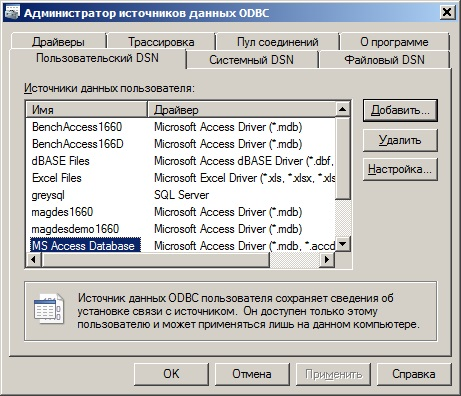
\includegraphics[width=0.5\linewidth]{bd_odbc_1.jpg}}
	\end{figure}
	
	\item Жмем \textit{<<Добавить>>} и выбираем драйвер \textit{<<Microsoft Access Driver (*.mdb, *accdb)>>}.
	
	\begin{figure}[H]
		\center{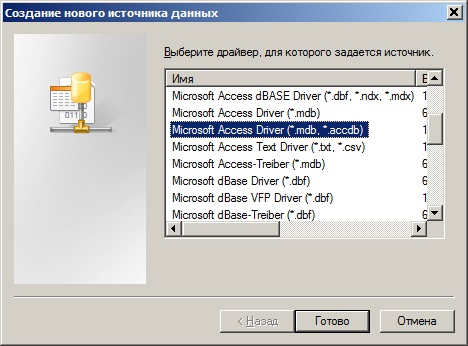
\includegraphics[width=0.5\linewidth]{bd_odbc_2.jpg}}
	\end{figure}
	
	\info{ Если данный пункт отсутствует, необходимо установить \textbf{Microsoft Access}.}
	
	\item Жмем \textit{<<Готово>>}, в~открывшейся форме выбираем необходимую \textbf{БД} и заполняем поля.
	
	\begin{figure}[H]
		\center{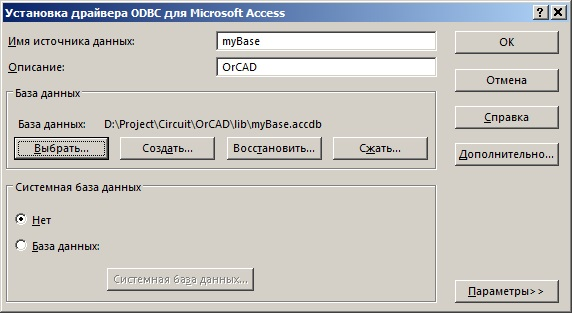
\includegraphics[width=0.5\linewidth]{bd_odbc_3.jpg}}
	\end{figure}
	
	\item Жмем \textit{<<OK>>} и проверяем что база появилась в списке.
\end{enumerate}



%%%------- Настройка multi-value полей
\subsubsection{Настройка multi-value полей} \label{sssec:bd_multi_value}

Начиная с версии \textbf{16.6}, каждое поле \textbf{БД} может являться multi-value.

Для этого необходимо поместить в автозагрузку скриптов: \\
\textit{C:/SPB\_Data-Silent/cdssetup/OrCAD\_Capture/tclscripts/capAutoLoad} или \\
\textit{C:/Cadence/SPB\_16.6/tools/capture/tclscripts/capAutoLoad}), \\
файл \textit{*.tcl} со следующим содержимым:
\lstinputlisting[language=tcl]{OrCAD/CISRowColor.tcl}	% листинг файла



%%%------- Подключение в CIS
\subsubsection{Подключение в CIS} \label{sssec:bs_setup_cis}



%%-------
\subsection{Вариантные исполнения} \label{ssec:variant_list}



%%%-------
\subsubsection{Передача в PCB Editor} \label{sssec:export_variant_list}

Передача вариантных исполнений их~схемного редактора в~редактор печатных плат, осуществляется в~несколько шагов:
\begin{enumerate}
	\item Запустить \textbf{Design Entry CIS};
	
	\item Перейти в~окно \textit{Part Manager};
	
	\item Сформировать список вариантных исполнений \textit{<<Menu -> Tools -> Export Variant List>>}; 
	
	\item Запустить \textbf{PCB Editor};
	
	\item Перейти в~окно \textit{<<Menu -> Manufacture -> Variants -> Create Assembly Drawing...>>};
	
	\item Выбрать нужные настройки и вариант исполнения.
	
		\begin{figure}[H]
			\center{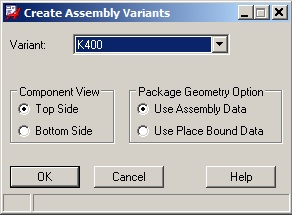
\includegraphics{create_assembly_variants.jpg}}
%			\caption{Окно вариантного исполнения} 
%			\label{fig:create_assembly_variants}
		\end{figure}	
	
\end{enumerate}

После этих действий появится новый подкласс в~классе \textit{Manufacture}. Для настроек установленных выше это будет \textit{<<Manufacture/K400\_Top>>}.